\section{Einarbeitung}
In der Einarbeitungsphase haben wir uns zunächst für eine Hadoop-Arbeitsumgebung entschieden. Da die meisten Projektteilnehmer über lediglich vier Gigabyte Arbeitsspeicher verfügen, fiel unsere Wahl auf die ressourcenschonende Hortonworks Sandbox\footnote{\url{http://hortonworks.com/products/hortonworks-sandbox/}}, die bei allen Teilnehmern problemlos ausgeführt werden konnte. Unter Verwendung der Sandbox haben wir den Umgang mit dem Hadoop-Ecosystem gelernt und erste Map/Reduce-Jobs ausgeführt. Darüber hinaus konnten wir weitere Tools wie Hive und Pig verwenden.

\renewcommand{\arraystretch}{1.3}

\subsection{Datenmodell}
Abbildung \ref{fig:ShoppersTables} zeigt das Datenmodell, dass aus den Entitäten "`transactions"', "`history"', "'offers"', und "`submissions"' besteht. 

\begin{figure}[H]
\centering
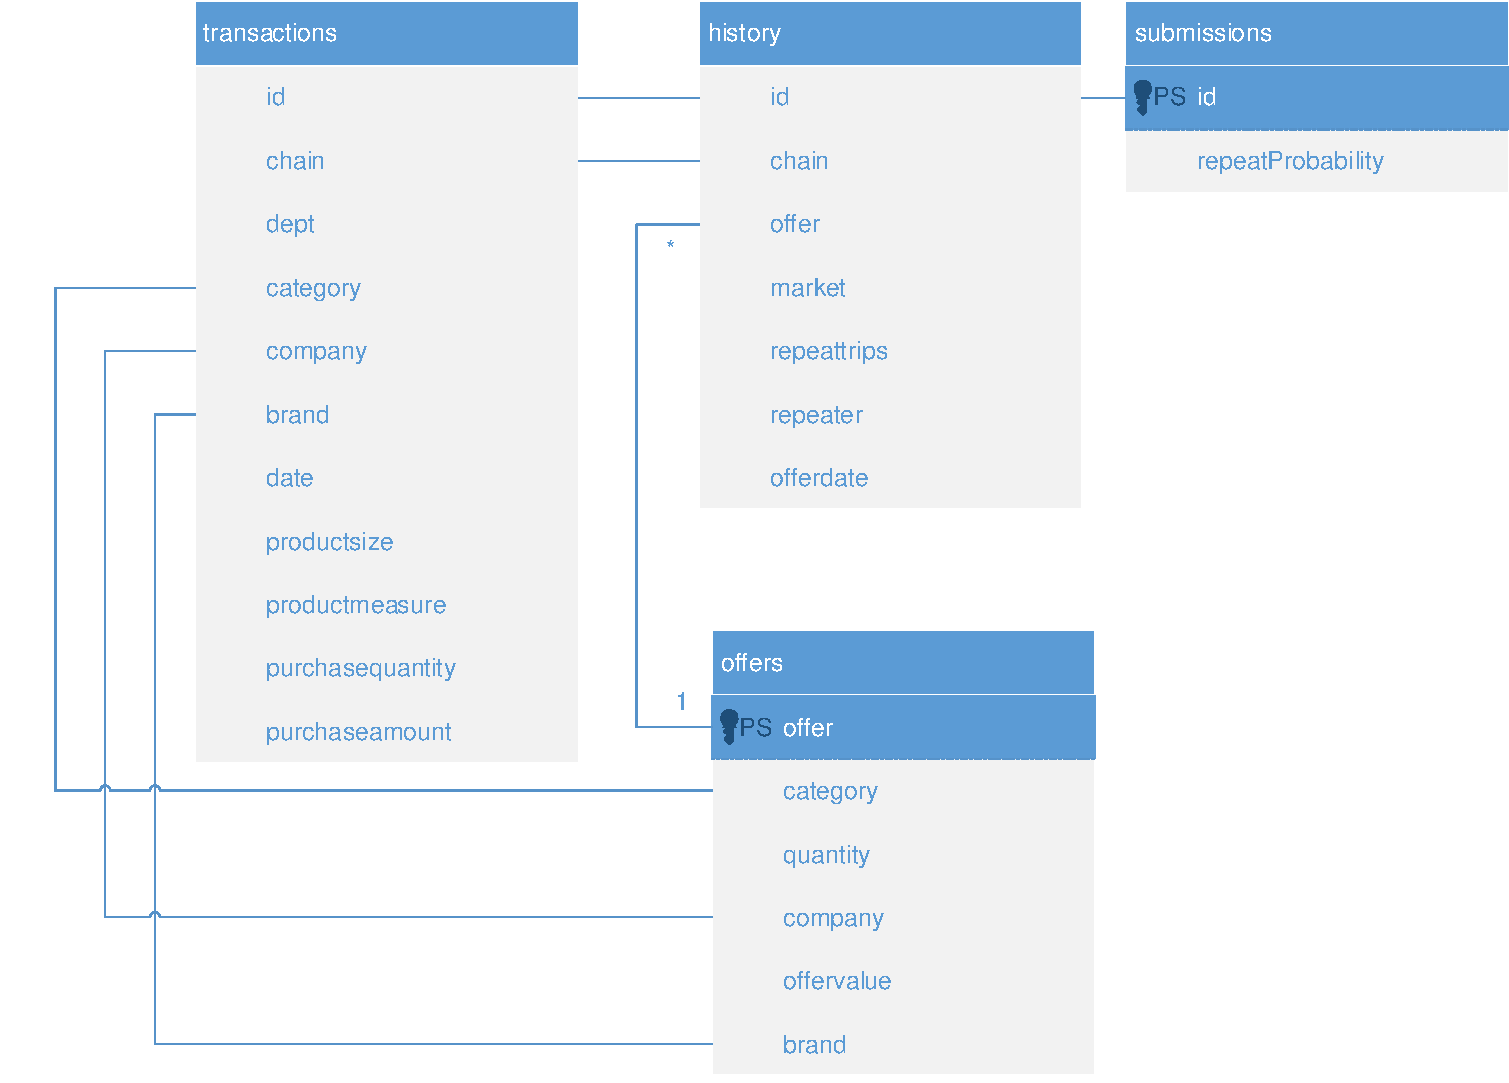
\includegraphics[width=0.9\linewidth]{Bilder/ShoppersTables}
\caption{Das Datenmodell der Shoppers-Challenge}
\label{fig:ShoppersTables}
\end{figure}

In den "`transactions"' (s. Tabelle \ref{tab:transactions}) stehen die Einkäufe der Kunden.
Die "`offers"' (s. Tabelle \ref{tab:offers}) enthalten Gutscheine, die an den Kunden verteilt wurden.
In der "`train\_history"' (s. Tabelle \ref{tab:trainhistory}) sind Informationen über die angebotenen Coupons enthalten.
Die "`test\_history"' entspricht der "`train\_history"' mit dem Unterschied, dass die beiden Felder "`repeattrips"' und "`repeater"' fehlen. Diese sind absichtlich nicht enthalten, da eine Vorhersage über diese Werte getroffen werden soll.
Die "`submissions"' (s. Tabelle \ref{tab:submissions}) enthalten die Ergebnisse, die wir bei Kaggle einreichen. Dabei wird einem Kunden eine Wiederkaufswahrscheinlichkeit zugeordnet.

Ziel dieses Projekts ist es, die Daten aus den "`transactions"', "`offers"' sowie der beiden Historiendaten zur Generierung von "`submissions"' zu nutzen. Es sollen Vorhersagen für alle Kunden-IDs aus der "`test\_history"' gemacht werden.

\begin{table}[h]
\centering
\begin{tabular}{l|l}
	 \textbf{Feld} & \textbf{Bedeutung}  \\ 
	\hline id & ID des Kunden \\ 
	\hline chain & ID der Marktkette \\ 
	\hline dept  & ID der Produktoberkategorie (z.B. Elektronikgeräte)  \\ 
	\hline category & ID der Produktkategorie (z.B. Smartphones) \\ 
	\hline company & ID der Firma die das Produkt verkauft \\ 
	\hline brand & ID der Marke (z.B. iPhone) \\ 
	\hline date & Kaufdatum \\
	\hline productsize & Menge die gekauft wurde (2L Wasser, 500g Mehl) \\ 	
	\hline productmeasure & Einheit (Liter, Gramm, Stück) \\ 	
	\hline purchasequantity & Stückzahl die gekauft wurde (Drei 2L Flaschen Wasser)
	\vspace{0.3cm} \\ 
\end{tabular}
\caption{transactions}
\label{tab:transactions}
\end{table}

\begin{table}[h]
\centering
\begin{tabular}{l|l}
	\textbf{Feld} & \textbf{Bedeutung}  \\ 
	\hline offer & ID des Coupon \\ 
	\hline category & ID der Produktkategorie \\ 
	\hline quantity & Stückzahl ab der ein Coupon gilt \\ 
	\hline company & ID der Firma die Coupons anbietet \\ 
	\hline offervalue & Preis \\ 
	\hline brand & ID der Marke
	\vspace{0.3cm} \\ 
\end{tabular}
\caption{offers}
\label{tab:offers}
\end{table}

\begin{table}[h]
\centering
\begin{tabular}{l|l}
	\textbf{Feld} & \textbf{Bedeutung}  \\ 
	\hline id & ID des Kunden \\ 
	\hline chain & ID der Marktkette \\ 
	\hline offer  & ID des Coupon  \\ 
	\hline market & ID der Region in der sich der Markt befindet  \\ 
	\hline repeattrips & Anzahl der Wiederholungskäufe (gleiches Produkt)  \\ 
	\hline repeater & Gibt an, ob repeattrips größer 0 ist \\ 
	\hline offerdate & Datum an dem der Kunde den Coupon erhalten hat 
	\vspace{0.3cm} \\ 
\end{tabular} 
\caption{train\_history}
\label{tab:trainhistory}
\end{table}

\begin{table}[h]
	\centering
\begin{tabular}{l|l}
	\textbf{Feld} & \textbf{Bedeutung}  \\ 
	\hline id & ID des Kunden \\ 
	\hline repeatProbability & Wahrscheinlichkeit das der Kunde erneut kauft 
	\vspace{0.3cm} \\
\end{tabular} 
\caption{submissions}
\label{tab:submissions}
\end{table}

\subsection{Technologieentscheidung}
Zu Beginn des Projekts haben wir uns Gedanken über die Auswahl der Technologien gemacht. Zum Zeitpunkt der Einarbeitungsphase haben wir bereits Hive und Pig durch gruppenübergreifende Vorträge kennen gelernt. Darüber hinaus standen uns keine weiteren Optionen zur Verfügung, da alternative Technologien erst zu einem späteren Zeitpunkt vorgestellt worden sind.

Somit beschränkte sich die Technologieentscheidung auf die Wahl zwischen Hive und Pig. Da wir in unserem Projekt ausschließlich Analysen auf strukturierte Daten durchgeführt haben, fiel unsere Entscheidung auf Hive. Der einfache Datenimport in Form von Tabellen und die einfachen Abfragemöglichkeiten in der SQL-ähnlichen Abfragesprache HQL waren die ausschlaggebenden Kriterien.

Die Technologien, die wir neben Hive verwendet haben, werden im weiteren Verlauf der Dokumentation erläutert.


\subsection{Data-Mining-Verfahren}
In diesem Kapitel werden wir einen Überblick über Data-Mining-Verfahren geben, die für das Kaggle-Projekt von uns genutzt wurden. Zuerst werden wir das Prinzip des Machine Learning erläutern. Anschließend werden die beiden Daten-Mining-Konzepte Regressionsanalyse und Klassifizierung vorgestellt. Zu letzt wird eine Überblick über die benutzten Werkzeuge zum Machine Learning gegeben.

\subsubsection{Machine Learning}
Die folgende Beschreibung aus Wikipedia beschreibt relativ genau welche Funktion Machine Learning hat. “Maschinelles Lernen ist ein Oberbegriff für die ‘künstliche’ Generierung von Wissen aus Erfahrung: Ein künstliches System lernt aus Beispielen und kann nach Beendigung der Lernphase verallgemeinern.”

Beim Machine Learning versucht man aus vorhanden Informationen ein Modell zu generieren, das eine Aussage über neue Informationen treffen kann. Die Informationen, die zur Erstellung des Modells genutzt werden, werden Trainingsdaten genannt. Informationen, über die eine Aussage getroffen werden soll, nennt man Testdaten.

\begin{figure}[H]
\centering
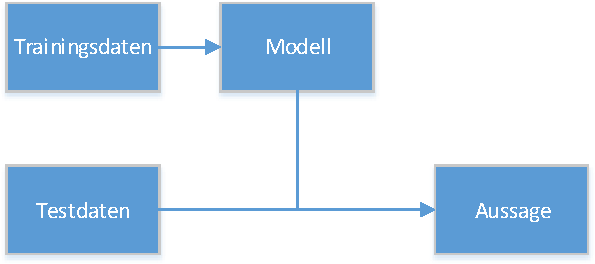
\includegraphics[width=0.9\linewidth]{Bilder/DataMining}
\caption{Machine Learning im Modell}
\label{fig:MachineLearning}
\end{figure}

Beim Kaggle-Projekt setzten sich die Trainingsdaten aus den Tabellen offers, transactions, trainHistory, für die Testdaten wird die Tabelle testHistory anstatt der Tabelle trainHistory genutzt. Das Modell soll eine Aussage darüber geben, ob ein Kunde erneut kaufen wird.

Es gibt 3 Kategorien beim Machine Learning, das Überwachte Lernen (supervised learning), das Unüberwachte Lernen (unsupervised learning) und das Bestärkende Lernen (reinforcement learning). Das Bestärkende Lernen ist das Lernen durch Belohnung und Bestrafung. Wir werden hier aber nicht weiter auf das Bestärkende Lernen eingehen.

Beim Überwachtem Lernen übergibt man einem Algorithmus Paare aus Eingabedaten und Funktionwerten. Der Algorithmus erstellt daraus ein Modell, das zu einer neuen Eingabe eine Aussage über den Funktionswert trifft. Beispiele für das Überwachte Lernen sind Regressionsanalyse und Klassifizierung.

Beim Unüberwachtem Lernen erzeugt ein Algorithmus ein Modell unter Betrachtung einer Menge von Eingabedaten. Dieses Modell soll dann eine Aussage über die Eingabedaten treffen. Das typische Beispiel für Unüberwachtes Lernen ist Clustering. Hierbei wird versucht Gruppen in der Menge der Eingabedaten zu finden.

Wir werden uns für das Kaggle-Projekt vor allen Dingen mit dem Überwachten Lernen beschäftigen. Denkbar sind zum einen eine Regressionsanalyse, zum anderen eine Binäre Klassifizierung.

Für das Kaggle-Projekt kann man sich eine Regressionsanalyse vereinfacht so vorstellen, dass man eine Menge von Eingabedaten hat und eine Funktion findet, die dafür einen Funktionwert zwischen 0 bis 1 generiert. Der Funktionswert soll die Wahrscheinlichkeit, dass ein Kunde erneut kauft, darstellen. Der Nachteil hierbei ist, dass bei den Trainingsdaten die Funktionswerte nur 0 oder 1 sind und keinen Wert dazwischen einnehmen kann.

Daher wäre eine Binäre Klassifizierung ein anderer möglicher Ansatz. Die beiden möglichen Klassen sind hierbei 0 und 1. 0 für Kunde kauft nicht erneut und 1 für Kunde kauft erneut. Der Algorithmus soll hier ein Aussage treffen zu welcher Wahrscheinlichkeit ein Testdatensatz zur Klasse 0 oder zur Klasse 1 gehört.

Bei Regressionsanalyse und Klassifizierung gibt es das Problem der Überanpassung (overfitting). Von Overfitting spricht man, wenn ein Algorithmus die Trainingsdaten auswendig gelernt hat, aber keine Funktion erstellt hat, die die Verbindungen in den Datensätzen darstellt. Zur Verhinderung von Overfitting übergibt man nur die wichtigen bzw. relevanten Daten an den Algorithmus zur Erstellung des Modells. Die Einschränkung der Daten nennt man auch feature selection.

\subsubsection{Online/Offline Machine Learning}

Beim Machine Learning gibt es zwei verschiedene Ansätze, zum einen das Online Machine Learning und zum anderen das Offline Machine Learning. Beim Online Machine Learning nimmt der Algorithmus schrittweise je einen Datensatz aus den Trainingsdaten. Der Algorithmus passt daraufhin das Modell an und nimmt den nächsten Datensatz. Daher ist beim Online Machine Learning das Modell erweitert werden. Dies ist zum Beispiel dann nützlich wenn man ein Modell über Trainingsdaten der letzten Jahre hat und diese um die Daten der letzten Tage erweitern will. Der Nachteil hierbei ist allerdings, dass die Reihenfolge, in der die Trainingsdaten eingelesen werden, Einfluss auf das Modell nimmt. Beim Offline Machine Learning kann man nur einmal Trainingsdaten übergeben, diese werden dann unabhängig von der Reihenfolge verarbeitet.

\begin{table}[h]
	\centering
\begin{tabular}{l|c|c}
	\textbf{} \textbf{Offline learning} & \textbf{Online learning}  \\ 
	\hline id & ID des Kunden \\ 
	\hline repeatProbability & Wahrscheinlichkeit das der Kunde erneut kauft 
	\vspace{0.3cm} \\
\end{tabular} 
\caption{submissions}
\label{tab:submissions}
\end{table}

 
Implementierungen

In diesem Kapitel werden wir verschiedene Implementierungen für Machine Learning, die für das Kaggle-Projekt in Frage kommen, vorstellen.

Vowpal Wabbit

Vowpal Wabbit ist ein Open-Source Programm für Online Machine Learning. Es wurde ursprünglich bei Yahoo! Research und zur zeit wird es bei Microsoft Research entwickelt. Es bietet die Möglichkeit Klassifizierung und Regressions Algorithmen zu nutzen. Die typische Nutzung von Vowpal Wabbit ist über die Kommandozeile.

Mahout

Apache Mahout ist eine Projekt zur Implementierung von Machine Learning, das vor allen Dingen auf Collaborative Filtering, Clustering und Klassifikation fokussiert ist. Die meisten Implementierungen in Mahout setzten auf Hadoop auf und nutzen das Map/Reduce-Verfahren. Außerdem ist eine Einbindung von Mahout in AWS relative einfach.

Glmnet

Glmnet ist ein R-Package das Lineare und Logistische Regression implementiert.


In der folgenden Tabelle sollen die möglichen Anwendungsumgebungen der Implementierungen dargestellt werden.



HDFS (Hortonworks)
AWS
Lokal
Vowpal Wabbit




✔
Apache Mahout
✔
✔
✔
Glmnet
✔
✔
✔

